\chapter{Logische Gatter}\label{ch:logische_gatter}

\section{Vom Stromkreis zur Information}

Wir wissen aus \cref{ch:zahlendarstellungen,ch:kodierungen} bereits, dass sich beliebige Informationen -- Zahlen, Buchstaben, Bilder -- als Folgen von \tib{Bits}\index{Bit} darstellen lassen (vgl. \cref{mydefinition:bit-byte}). Nun wollen wir der Frage nachgehen, wie ein Computer diese Nullen und Einsen tatsächlich \emph{physikalisch} verarbeitet. Wir starten dazu bei der Hardware: Ein Chip ist zunächst ein Netzwerk aus leitenden Verbindungen und schaltenden Bauelementen. Die zentrale Idee lautet: \textbf{Elektrische Zustände werden als logische Zustände interpretiert}.

\begin{figure}[H]
    \centering
    \begin{tikzpicture}[scale=1.0]
    \begin{scope}[shift={(0,0)}, local bounding box=openBB]
        \coordinate (open-base) at (0,0);
        \coordinate (open-bat-bot) at ($(open-base)+(0.6,0.8)$);
        \coordinate (open-bat-top) at ($(open-base)+(0.6,2.2)$);
        \coordinate (open-sw-left) at ($(open-base)+(2.0,2.2)$);
        \coordinate (open-sw-right) at ($(open-base)+(2.9,2.2)$);
        \coordinate (open-lamp) at ($(open-base)+(3.8,2.2)$);
        \coordinate (open-ret) at ($(open-base)+(3.8,0.8)$);

        \draw (open-bat-bot) -- (open-bat-top);
        \draw ($(open-base)+(0.45,1.15)$) -- ($(open-base)+(0.75,1.15)$);
        \draw ($(open-base)+(0.50,1.60)$) -- ($(open-base)+(0.70,1.60)$);
        \node[left] at ($(open-base)+(0.35,1.35)$) {$U$};

        \draw (open-bat-top) -- (open-sw-left);
        \draw (open-sw-left) -- ($(open-sw-left)+(0.6,0.3)$);
        \draw (open-sw-right) -- (open-lamp);
        \draw (open-lamp) circle (0.35);
        \draw ($(open-base)+(3.55,1.95)$) -- ($(open-base)+(4.05,2.45)$);
        \draw (open-bat-bot) -- (open-ret) -- ($(open-lamp)+(0,-0.35)$);

        \node at ($(open-base)+(2.35,2.65)$) {\tiny kein Kontakt};
        \node at ($(open-base)+(3.8,1.3)$) {Last aus};
        \node at ($(open-base)+(2.5,2.95)$) {Schalter offen};
    \end{scope}
    \node[draw,rounded corners,fit=(openBB),inner sep=8pt] {};

    \begin{scope}[shift={(6.2,0)}, local bounding box=closedBB]
        \coordinate (closed-base) at (0,0);
        \coordinate (closed-bat-bot) at ($(closed-base)+(0.6,0.8)$);
        \coordinate (closed-bat-top) at ($(closed-base)+(0.6,2.2)$);
        \coordinate (closed-sw-left) at ($(closed-base)+(2.0,2.2)$);
        \coordinate (closed-sw-right) at ($(closed-base)+(2.6,2.2)$);
        \coordinate (closed-lamp) at ($(closed-base)+(3.8,2.2)$);
        \coordinate (closed-ret) at ($(closed-base)+(3.8,0.8)$);

        \draw (closed-bat-bot) -- (closed-bat-top);
        \draw ($(closed-base)+(0.45,1.15)$) -- ($(closed-base)+(0.75,1.15)$);
        \draw ($(closed-base)+(0.50,1.60)$) -- ($(closed-base)+(0.70,1.60)$);
        \node[left] at ($(closed-base)+(0.35,1.35)$) {$U$};

        \draw (closed-bat-top) -- (closed-sw-left);
        \fill (closed-sw-left) circle (0.04);
        \fill (closed-sw-right) circle (0.04);
        \draw[line width=0.5pt] (closed-sw-left) -- (closed-sw-right);
        \draw (closed-sw-right) -- (closed-lamp);
        \draw (closed-lamp) circle (0.35);
        \fill (closed-lamp) circle (0.12);
        \draw (closed-bat-bot) -- (closed-ret) -- ($(closed-lamp)+(0,-0.35)$);

        \node at ($(closed-base)+(2.3,2.65)$) {\tiny Kontakt};
        \node at ($(closed-base)+(3.8,1.3)$) {Last aktiv};
        \node at ($(closed-base)+(2.5,2.95)$) {Schalter geschlossen};
    \end{scope}
    \node[draw,rounded corners,fit=(closedBB),inner sep=8pt] {};
\end{tikzpicture}

    \caption{Grundidee eines elektrischen Schaltnetzes: Kontakt \enquote{offen} oder \enquote{geschlossen}.}
    \label{fig:stromkreis_grundidee}
\end{figure}

Ob Strom fliesst oder nicht, hängt davon ab, ob ein leitender Pfad existiert. In der Digitaltechnik werden solche physikalischen Zustände auf zwei logische Zustände abgebildet:
\[
    \text{niedrige Spannung} \longleftrightarrow 0,
    \qquad
    \text{hohe Spannung} \longleftrightarrow 1.
\]

\begin{myremark}[Warum ausgerechnet zwei Zustände?]
    Wie wir in \cref{ch:zahlendarstellungen} gesehen haben, liesse sich eine Schaltung im Prinzip auch mit mehr als zwei Spannungspegeln realisieren (analog zu einem $b$-adischen Zahlensystem mit $b>2$). In der Praxis hat sich jedoch das Binärsystem durchgesetzt, da zwei klar unterscheidbare Zustände (\enquote{Strom fliesst} / \enquote{Strom fliesst nicht}) sehr zuverlässig und störungsresistent erkannt werden können.
\end{myremark}

Wichtig ist: In echten Schaltungen gibt es Rauschen, Verzögerungen und Fertigungstoleranzen. Deshalb arbeitet man mit \textbf{Spannungsbereichen} statt mit exakt einem Wert. Typisch ist zum Beispiel:
\begin{itemize}
    \item $0$ wird zuverlässig erkannt, wenn die Eingangsspannung hinreichend klein ist (nahe $0\,\mathrm{V}$),
    \item $1$ wird zuverlässig erkannt, wenn die Eingangsspannung hinreichend gross ist (nahe Versorgungsspannung, z.B. $3{,}3\,\mathrm{V}$ oder $5\,\mathrm{V}$).
\end{itemize}

\section{Vom Transistor zum Gatter}

In modernen Mikroprozessoren übernehmen \tib{Transistoren}\index{Transistor} die Rolle extrem schneller, rein elektronischer Schalter. Im Gegensatz zu mechanischen Lichtschaltern besitzen Transistoren keine beweglichen Teile, sondern werden durch eine elektrische Steuerspannung geschaltet:
\begin{itemize}
    \item \textbf{Steuersignal = 1 (Spannung liegt an)}: Der Schalter ist \textbf{geschlossen} (Strom fliesst).
    \item \textbf{Steuersignal = 0 (keine Spannung)}: Der Schalter ist \textbf{offen} (Strompfad ist unterbrochen).
\end{itemize}

Ein logisches \tib{Gatter}\index{Gatter} fasst eine Schaltung aus solchen Schaltern zu einem standardisierten Baustein zusammen: Es nimmt ein oder mehrere digitale Eingangssignale entgegen und liefert ein klares Ausgangssignal ($0$ oder $1$). In den folgenden Abschnitten betrachten wir für jeden Gattertyp sein logisches Verhalten (Wahrheitstabelle), sein genormtes Schaltzeichen und seine anschauliche Umsetzung als elektrische Schaltung.

\begin{myremark}[Exkurs: CMOS-Technologie in modernen Halbleiterchips]
    In echten Mikrochips (wie der CPU in Smartphones oder Computern) verwendet man die sogenannte \gls{CMOS}-Technologie (\textit{Complementary Metal-Oxide-Semiconductor}). Dabei arbeiten zwei gegensätzliche Transistortypen (p- und n-Kanal-Transistoren) paarweise als komplementäre Schalter: Der eine schliesst bei $0$ die Verbindung zur Versorgungsspannung ($V_{\text{DD}} = 1$), der andere bei $1$ die Verbindung zur Masse ($0\,\text{V} = 0$). Durch diese komplementäre Anordnung fliesst im ruhenden Zustand fast kein Strom.
\end{myremark}

\begin{mydefinition}[Hardware-relevante Kennwerte]
    Reale Gatter werden nicht nur durch ihre Wahrheitstabelle beschrieben, sondern auch durch technische Kennwerte:
    \begin{itemize}
        \item \tib{Propagationsverzögerung}\index{Propagationsverzögerung}: Zeit zwischen Eingangsänderung und stabiler Ausgangsänderung.
        \item \tib{Leistungsaufnahme}\index{Leistungsaufnahme}: Energiebedarf durch Schalten und Leckströme.
        \item \tib{Fan-out}\index{Fan-out}: Anzahl von Eingängen, die ein Ausgang zuverlässig treiben kann.
    \end{itemize}
\end{mydefinition}

\section{Logische Grundverknüpfungen}

Die Grundlage aller Rechenoperationen eines Computers bilden \tib{Boolesche Funktionen}\index{Boolesche Funktion}: Funktionen, die ein oder mehrere Bits als Eingabe erhalten und genau ein Bit als Ausgabe liefern.

\subsection{NOT -- Negation (Inverter)}

\begin{mydefinition}[NOT-Gatter]
    Das \textbf{NOT-Gatter} (Inverter) hat \emph{einen} Eingang $x$ und kehrt dessen Signal um:
    \[
        \overline{0} = 1, \qquad \overline{1} = 0.
    \]
\end{mydefinition}

\begin{figure}[H]
    \centering
    \begin{tikzpicture}[circuit logic US, scale=1.3]
    \node[not gate, draw] (not1) {};
    \draw (not1.input) ++(-0.7,0) -- (not1.input) node[left] {$x$};
    \draw (not1.output) -- ++(0.7,0) node[right] {$\overline{x}$};
\end{tikzpicture}

    \caption{Symbol des NOT-Gatters.}
    \label{fig:not_gatter}
\end{figure}

\begin{table}[H]
    \centering
    \begin{tabular}{cc}
        $x$ & $\overline{x}$ \\\midrule\midrule
        0 & 1 \\\midrule
        1 & 0 \\
    \end{tabular}
    \caption{Wahrheitstabelle des NOT-Gatters.}
    \label{tab:not}
\end{table}

\begin{figure}[H]
    \centering
    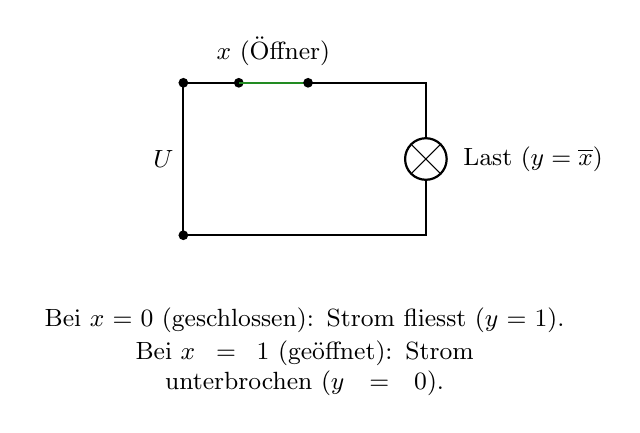
\begin{tikzpicture}[scale=0.88, >=stealth]
        \draw[thick] (0,0) -- (0,2.2) -- (0.8,2.2);
        \node[left, font=\small] at (0,1.1) {$U$};
        \fill (0,0) circle (2pt); \fill (0,2.2) circle (2pt);
        
        % Öffner-Schalter x
        \fill (0.8, 2.2) circle (2pt);
        \draw[thick, ForestGreen] (0.8, 2.2) -- (1.8, 2.2);
        \node[above, font=\small] at (1.3, 2.3) {$x$ (Öffner)};
        \fill (1.8, 2.2) circle (2pt);
        \draw[thick] (1.8, 2.2) -- (3.5, 2.2) -- (3.5, 1.4);
        
        % Lampe y
        \draw[thick] (3.5, 1.1) circle (0.3);
        \draw (3.3, 0.9) -- (3.7, 1.3);
        \draw (3.3, 1.3) -- (3.7, 0.9);
        \node[right, font=\small] at (3.9, 1.1) {Last ($y = \overline{x}$)};
        \draw[thick] (3.5, 0.8) -- (3.5, 0) -- (0,0);
        
        \node[align=center, font=\small, text width=6.8cm, anchor=north] at (1.75, -0.9) {Bei $x=0$ (geschlossen): Strom fliesst ($y=1$).\\[1pt]Bei $x=1$ (geöffnet): Strom unterbrochen ($y=0$).};
    \end{tikzpicture}
    \caption{Elektrische Schaltung für NOT: Ruhekontakt (Öffner).}
    \label{fig:not_schaltung}
\end{figure}

\begin{myremark}[Erinnerung: Symbole elektrischer Schaltungen]
    In den Ersatzschaltbildern werden folgende Symbole verwendet:
    \begin{itemize}
        \item \textbf{$U$ (Elektrische Spannung):} Steht für die \emph{Spannungsquelle} (z.\,B. Batterie oder Netzteil), welche den Stromkreis speist.
        \item \textbf{Last / Lampe ($\otimes$):} Elektrischer Verbraucher. Leuchtet die Lampe, ist das Ausgangssignal $y=1$.
    \end{itemize}
\end{myremark}

\begin{myremark}[Schalterarten: Schliesser (Arbeitskontakt) vs. Öffner (Ruhekontakt)]
    In den Schaltungsdiagrammen kommen zwei grundlegende Schalterarten zum Einsatz:
    \begin{center}
        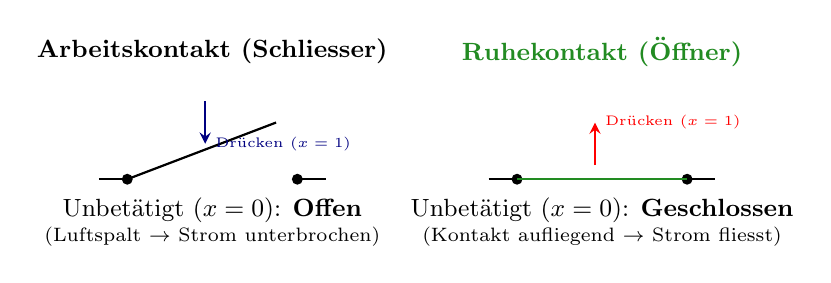
\begin{tikzpicture}[scale=0.9, >=stealth]
            % --- Arbeitskontakt (Schliesser) ---
            \begin{scope}[shift={(0,0)}]
                \node[font=\small\bfseries] at (1.2, 1.8) {Arbeitskontakt (Schliesser)};
                % Anschlüsse und Festkontakte
                \draw[thick] (-0.4,0) -- (0,0); \fill (0,0) circle (2.2pt);
                \draw[thick] (2.4,0) -- (2.8,0); \fill (2.4,0) circle (2.2pt);
                
                % Schalterhebel offen
                \draw[thick] (0,0) -- (2.1, 0.8);
                \draw[->, thick, NavyBlue] (1.1, 1.1) -- (1.1, 0.5) node[right, font=\tiny] {Drücken ($x=1$)};
                
                \node[font=\small, align=center] at (1.2, -0.6) {Unbetätigt ($x=0$): \textbf{Offen}\\[-2pt]{\scriptsize(Luftspalt $\rightarrow$ Strom unterbrochen)}};
            \end{scope}
            
            % --- Ruhekontakt (Öffner) ---
            \begin{scope}[shift={(5.5,0)}]
                \node[font=\small\bfseries, ForestGreen] at (1.2, 1.8) {Ruhekontakt (Öffner)};
                % Anschlüsse und Festkontakte
                \draw[thick] (-0.4,0) -- (0,0); \fill (0,0) circle (2.2pt);
                \draw[thick] (2.4,0) -- (2.8,0); \fill (2.4,0) circle (2.2pt);
                
                % Schalterhebel aufliegend (geschlossen)
                \draw[thick, ForestGreen] (0,0) -- (2.4,0);
                \draw[->, thick, Red] (1.1, 0.2) -- (1.1, 0.8) node[right, font=\tiny] {Drücken ($x=1$)};
                
                \node[font=\small, align=center] at (1.2, -0.6) {Unbetätigt ($x=0$): \textbf{Geschlossen}\\[-2pt]{\scriptsize(Kontakt aufliegend $\rightarrow$ Strom fliesst)}};
            \end{scope}
        \end{tikzpicture}
    \end{center}
    \begin{itemize}
        \item \textbf{Arbeitskontakt (Schliesser):}
            \begin{itemize}
                \item \emph{Unbetätigt ($x=0$)}: Schalter ist \textbf{offen} $\rightarrow$ Stromkreis unterbrochen.
                \item \emph{Betätigt ($x=1$)}: Schalter wird \textbf{geschlossen} $\rightarrow$ Strom fliesst.
                \item \emph{Beispiele}: Standard-Lichtschalter, Türklingel, Tastatur-Tasten.
            \end{itemize}
        \item \textbf{Ruhekontakt (Öffner, \textcolor{ForestGreen}{grün}):}
            \begin{itemize}
                \item \emph{Unbetätigt ($x=0$)}: Schalter ist \textbf{geschlossen} $\rightarrow$ Strom fliesst dauerhaft.
                \item \emph{Betätigt ($x=1$)}: Schalter wird \textbf{geöffnet} $\rightarrow$ Stromkreis unterbrochen.
                \item \emph{Beispiele}: Not-Aus-Schalter, Alarmanlagen-Fensterkontakte (Ruhestromprinzip).
            \end{itemize}
    \end{itemize}
\end{myremark}

\begin{myremark}[Exkurs: Umsetzung des NOT-Gatters in CMOS-Technologie]
    In modernen Mikroprozessoren werden logische Gatter nicht mit mechanischen Schaltern, sondern mit zwei gegensätzlich schaltenden Transistoren (CMOS) umgesetzt:
    \begin{center}
        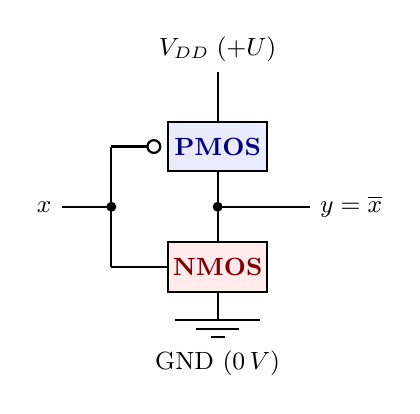
\begin{tikzpicture}[scale=0.9, >=stealth]
            % Versorgung oben (VDD)
            \draw[thick] (2,3.1) node[above, font=\small] {$V_{DD} \; (+U)$} -- (2,2.4);
            
            % PMOS oben (p-Kanal Transistor)
            \draw[thick, fill=blue!8] (1.3,1.7) rectangle (2.7,2.4);
            \node[font=\small\bfseries, color=NavyBlue] at (2,2.05) {PMOS};
            \draw[thick] (1.1,2.05) circle (0.09cm); % Invertierungskreis
            \draw[thick] (0.5,2.05) -- (1.01,2.05);
            
            % Verbindung zwischen PMOS und NMOS
            \draw[thick] (2,1.7) -- (2,0.7);
            \draw[thick] (2,1.2) -- (3.3,1.2) node[right, font=\small] {$y = \overline{x}$};
            \fill (2,1.2) circle (2pt);
            
            % NMOS unten (n-Kanal Transistor)
            \draw[thick, fill=red!8] (1.3,0) rectangle (2.7,0.7);
            \node[font=\small\bfseries, color=Maroon] at (2,0.35) {NMOS};
            \draw[thick] (0.5,0.35) -- (1.3,0.35);
            
            % Masse unten (GND)
            \draw[thick] (2,0) -- (2,-0.4);
            \draw[thick] (1.4,-0.4) -- (2.6,-0.4);
            \draw[thick] (1.7,-0.52) -- (2.3,-0.52);
            \draw[thick] (1.9,-0.64) -- (2.1,-0.64);
            \node[below, font=\small] at (2,-0.7) {GND ($0\,\text{V}$)};
            
            % Eingang x
            \draw[thick] (0.5,2.05) -- (0.5,0.35);
            \draw[thick] (-0.2,1.2) node[left, font=\small] {$x$} -- (0.5,1.2);
            \fill (0.5,1.2) circle (2pt);
        \end{tikzpicture}
    \end{center}
    Die beiden Transistoren wirken als komplementäres Schalterpaar:
    \begin{itemize}
        \item \textbf{Eingang $x = 0$ ($0\,\text{V}$)}: PMOS (oben) schliesst, NMOS (unten) öffnet $\rightarrow$ Ausgang $y$ wird mit $V_{DD}$ verbunden $\rightarrow \mathbf{y = 1}$.
        \item \textbf{Eingang $x = 1$ ($+U$)}: PMOS (oben) öffnet, NMOS (unten) schliesst $\rightarrow$ Ausgang $y$ wird mit GND verbunden $\rightarrow \mathbf{y = 0}$.
    \end{itemize}
\end{myremark}

\begin{myexercise}
    Eine Alarmanlage arbeitet nach dem Ruhestrom-Prinzip: Ein Fensterkontakt liefert im ungestörten Zustand $x=1$ (geschlossen). Wird der Draht durchtrennt oder das Fenster geöffnet, fällt das Signal auf $x=0$.
    \begin{enumerate}[(a)]
        \item Welches Gatter wird benötigt, damit die Alarmlampe $y$ bei Unterbrechung ($x=0$) aufleuchtet ($y=1$)?
        \item Geben Sie die zugehörige Wahrheitstabelle an.
    \end{enumerate}
    \begin{myanswer}
        \begin{enumerate}[(a)]
            \item Ein \textbf{NOT-Gatter} (Inverter), da $y = \overline{x}$.
            \item Wahrheitstabelle: $x=1 \Rightarrow y=0$ (kein Alarm); $x=0 \Rightarrow y=1$ (Alarm!).
        \end{enumerate}
    \end{myanswer}
\end{myexercise}

\subsection{AND -- Konjunktion (UND)}

\begin{mydefinition}[AND-Gatter]
    Das \textbf{AND-Gatter} hat \emph{zwei} Eingänge $x$ und $y$ und liefert genau dann den Ausgang \texttt{1}, wenn \emph{beide} Eingänge \texttt{1} sind:
    \[
        x \wedge y = 1 \iff x = 1 \text{ und } y = 1.
    \]
\end{mydefinition}

\begin{figure}[H]
    \centering
    \begin{tikzpicture}[circuit logic US, scale=1.3]
    \node[and gate, draw] (and1) {};
    \draw (and1.input 1) ++(-0.7,0) -- (and1.input 1) node[left] {$x$};
    \draw (and1.input 2) ++(-0.7,0) -- (and1.input 2) node[left] {$y$};
    \draw (and1.output) -- ++(0.7,0) node[right] {$x \wedge y$};
\end{tikzpicture}

    \caption{Symbol des AND-Gatters.}
    \label{fig:and_gatter}
\end{figure}

\begin{table}[H]
    \centering
    \begin{tabular}{ccc}
        $x$ & $y$ & $x \wedge y$ \\\midrule\midrule
        0 & 0 & 0 \\\midrule
        0 & 1 & 0 \\\midrule
        1 & 0 & 0 \\\midrule
        1 & 1 & 1 \\
    \end{tabular}
    \caption{Wahrheitstabelle des AND-Gatters.}
    \label{tab:and}
\end{table}

\begin{figure}[H]
    \centering
    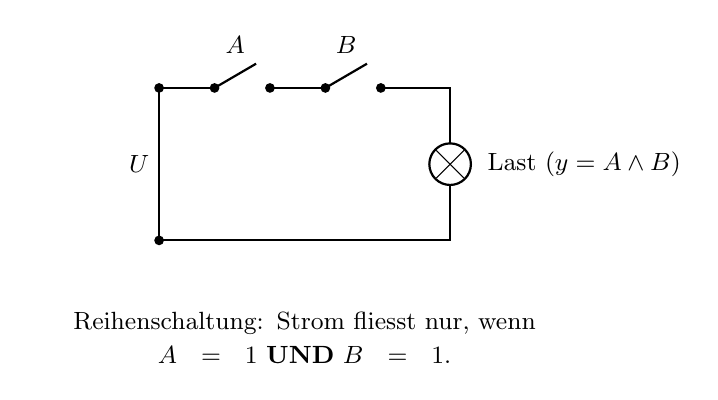
\begin{tikzpicture}[scale=0.88, >=stealth]
        \draw[thick] (0,0) -- (0,2.2) -- (0.8,2.2);
        \node[left, font=\small] at (0,1.1) {$U$};
        \fill (0,0) circle (2pt); \fill (0,2.2) circle (2pt);
        
        % Schalter A
        \fill (0.8, 2.2) circle (2pt);
        \draw[thick] (0.8, 2.2) -- (1.4, 2.55);
        \node[above, font=\small] at (1.1, 2.55) {$A$};
        \fill (1.6, 2.2) circle (2pt);
        \draw[thick] (1.6, 2.2) -- (2.4, 2.2);
        
        % Schalter B
        \fill (2.4, 2.2) circle (2pt);
        \draw[thick] (2.4, 2.2) -- (3.0, 2.55);
        \node[above, font=\small] at (2.7, 2.55) {$B$};
        \fill (3.2, 2.2) circle (2pt);
        \draw[thick] (3.2, 2.2) -- (4.2, 2.2) -- (4.2, 1.4);
        
        % Lampe y
        \draw[thick] (4.2, 1.1) circle (0.3);
        \draw (4.0, 0.9) -- (4.4, 1.3);
        \draw (4.0, 1.3) -- (4.4, 0.9);
        \node[right, font=\small] at (4.6, 1.1) {Last ($y = A \land B$)};
        \draw[thick] (4.2, 0.8) -- (4.2, 0) -- (0,0);
        
        \node[align=center, font=\small, text width=6.8cm, anchor=north] at (2.1, -0.9) {Reihenschaltung: Strom fliesst nur, wenn\\[1pt]\textbf{$A=1$ UND $B=1$}.};
    \end{tikzpicture}
    \caption{Elektrische Schaltung für AND: Reihenschaltung zweier Schalter.}
    \label{fig:and_schaltung}
\end{figure}

\begin{myexercise}
    Eine Stanze in einer Fabrik darf aus Sicherheitsgründen nur auslösen ($y=1$), wenn der Arbeiter \emph{gleichzeitig} mit der linken Hand Taster $A$ und mit der rechten Hand Taster $B$ drückt ($A=1$ und $B=1$).
    Erklären Sie, warum hier eine Reihenschaltung bzw. ein AND-Gatter zwingend erforderlich ist.
    \begin{myanswer}
        Wäre es eine Parallelschaltung (OR), könnte der Arbeiter einen Taster festklemmen und mit einer Hand in die Stanze greifen. Nur bei einer Reihenschaltung (AND) müssen zwingend beide Hände beide Taster bedienen.
    \end{myanswer}
\end{myexercise}

\subsection{OR -- Disjunktion (ODER)}

\begin{mydefinition}[OR-Gatter]
    Das \textbf{OR-Gatter} hat \emph{zwei} Eingänge $x$ und $y$ und liefert genau dann den Ausgang \texttt{1}, wenn \emph{mindestens einer} der Eingänge \texttt{1} ist:
    \[
        x \vee y = 1 \iff x = 1 \text{ oder } y = 1.
    \]
\end{mydefinition}

\begin{figure}[H]
    \centering
    \begin{tikzpicture}[circuit logic US, scale=1.3]
    \node[or gate, draw] (or1) {};
    \draw (or1.input 1) ++(-0.7,0) -- (or1.input 1) node[left] {$x$};
    \draw (or1.input 2) ++(-0.7,0) -- (or1.input 2) node[left] {$y$};
    \draw (or1.output) -- ++(0.7,0) node[right] {$x \vee y$};
\end{tikzpicture}

    \caption{Symbol des OR-Gatters.}
    \label{fig:or_gatter}
\end{figure}

\begin{table}[H]
    \centering
    \begin{tabular}{ccc}
        $x$ & $y$ & $x \vee y$ \\\midrule\midrule
        0 & 0 & 0 \\\midrule
        0 & 1 & 1 \\\midrule
        1 & 0 & 1 \\\midrule
        1 & 1 & 1 \\
    \end{tabular}
    \caption{Wahrheitstabelle des OR-Gatters.}
    \label{tab:or}
\end{table}

\begin{figure}[H]
    \centering
    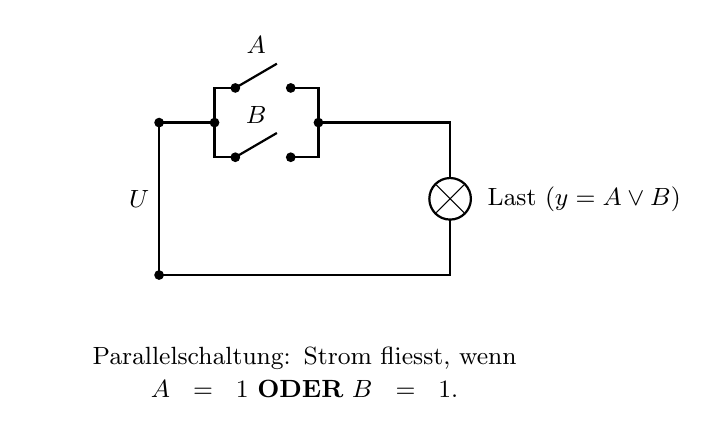
\begin{tikzpicture}[scale=0.88, >=stealth]
        \draw[thick] (0,0) -- (0,2.2) -- (0.8,2.2);
        \node[left, font=\small] at (0,1.1) {$U$};
        \fill (0,0) circle (2pt); \fill (0,2.2) circle (2pt);
        
        \draw[thick] (0.8, 2.2) |- (1.1, 2.7);
        \draw[thick] (0.8, 2.2) |- (1.1, 1.7);
        \fill (0.8, 2.2) circle (2pt);
        
        % Schalter A
        \fill (1.1, 2.7) circle (2pt);
        \draw[thick] (1.1, 2.7) -- (1.7, 3.05);
        \node[above, font=\small] at (1.4, 3.05) {$A$};
        \fill (1.9, 2.7) circle (2pt);
        \draw[thick] (1.9, 2.7) -| (2.3, 2.2);
        
        % Schalter B
        \fill (1.1, 1.7) circle (2pt);
        \draw[thick] (1.1, 1.7) -- (1.7, 2.05);
        \node[above, font=\small] at (1.4, 2.05) {$B$};
        \fill (1.9, 1.7) circle (2pt);
        \draw[thick] (1.9, 1.7) -| (2.3, 2.2);
        
        \fill (2.3, 2.2) circle (2pt);
        \draw[thick] (2.3, 2.2) -- (4.2, 2.2) -- (4.2, 1.4);
        
        % Lampe y
        \draw[thick] (4.2, 1.1) circle (0.3);
        \draw (4.0, 0.9) -- (4.4, 1.3);
        \draw (4.0, 1.3) -- (4.4, 0.9);
        \node[right, font=\small] at (4.6, 1.1) {Last ($y = A \lor B$)};
        \draw[thick] (4.2, 0.8) -- (4.2, 0) -- (0,0);
        
        \node[align=center, font=\small, text width=6.8cm, anchor=north] at (2.1, -0.9) {Parallelschaltung: Strom fliesst, wenn\\[1pt]\textbf{$A=1$ ODER $B=1$}.};
    \end{tikzpicture}
    \caption{Elektrische Schaltung für OR: Parallelschaltung zweier Schalter.}
    \label{fig:or_schaltung}
\end{figure}

\begin{myexercise}\label{myexercise:gatter-anwendung}
    Ein Fahrstuhl darf sich nur dann in Bewegung setzen, wenn die Tür geschlossen \emph{und} entweder das Übergewicht nicht überschritten ist \emph{oder} der Notfall-Modus deaktiviert ist. Modellieren Sie diese Bedingung mithilfe von AND-, OR- und NOT-Gattern und geben Sie die zugehörige logische Formel an.
    \begin{myanswer}
        Mit $t=$ \enquote{Tür geschlossen}, $u=$ \enquote{Übergewicht überschritten}, $n=$ \enquote{Notfall-Modus aktiv} lautet die Formel:
        \[
            t \wedge (\overline{u} \vee \overline{n}).
        \]
        Die Schaltung besteht aus zwei NOT-Gattern (für $\overline{u}$ und $\overline{n}$), einem OR-Gatter und einem abschliessenden AND-Gatter.
    \end{myanswer}
\end{myexercise}

\section{Weitere Gatter: NAND, NOR und XOR}

Aus den drei Grundverknüpfungen lassen sich weitere wichtige Gatter ableiten, die in der Praxis eine zentrale Rolle spielen.

\subsection{NAND -- Nicht-UND}

\begin{mydefinition}[NAND-Gatter]
    Das \tib{\gls{NAND}-Gatter}\index{NAND-Gatter} liefert die Negation des AND-Gatters:
    \[
        \overline{x \wedge y}.
    \]
    Es gibt genau dann \texttt{0} aus, wenn \emph{beide} Eingänge \texttt{1} sind; sonst immer \texttt{1}.
\end{mydefinition}

\begin{figure}[H]
    \centering
    \begin{tikzpicture}[circuit logic US, scale=1.3]
    \node[nand gate, draw] (nand1) {};
    \draw (nand1.input 1) ++(-0.7,0) -- (nand1.input 1) node[left] {$x$};
    \draw (nand1.input 2) ++(-0.7,0) -- (nand1.input 2) node[left] {$y$};
    \draw (nand1.output) -- ++(0.7,0) node[right] {$\overline{x \wedge y}$};
\end{tikzpicture}

    \caption{Symbol des NAND-Gatters (AND mit Kreis am Ausgang).}
    \label{fig:nand_gatter}
\end{figure}

\begin{table}[H]
    \centering
    \begin{tabular}{ccc}
        $x$ & $y$ & $\overline{x \wedge y}$ \\\midrule\midrule
        0 & 0 & 1 \\\midrule
        0 & 1 & 1 \\\midrule
        1 & 0 & 1 \\\midrule
        1 & 1 & 0 \\
    \end{tabular}
    \caption{Wahrheitstabelle des NAND-Gatters.}
    \label{tab:nand}
\end{table}

\begin{figure}[H]
    \centering
    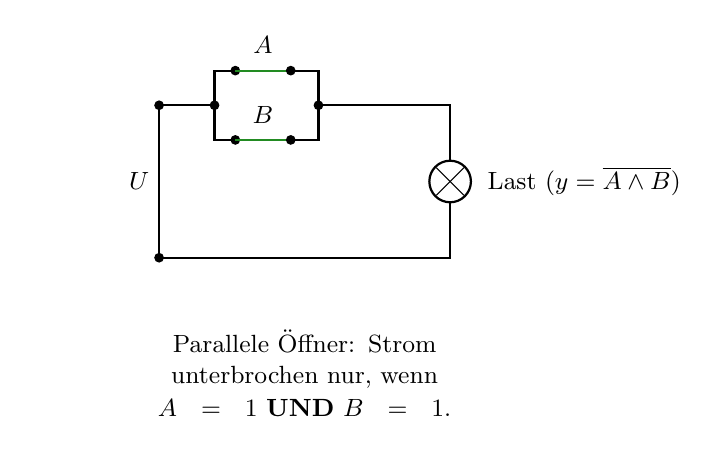
\begin{tikzpicture}[scale=0.88, >=stealth]
        \draw[thick] (0,0) -- (0,2.2) -- (0.8,2.2);
        \node[left, font=\small] at (0,1.1) {$U$};
        \fill (0,0) circle (2pt); \fill (0,2.2) circle (2pt);
        
        \draw[thick] (0.8, 2.2) |- (1.1, 2.7);
        \draw[thick] (0.8, 2.2) |- (1.1, 1.7);
        \fill (0.8, 2.2) circle (2pt);
        
        % Öffner A
        \fill (1.1, 2.7) circle (2pt);
        \draw[thick, ForestGreen] (1.1, 2.7) -- (1.9, 2.7);
        \node[above, font=\small] at (1.5, 2.8) {$A$};
        \fill (1.9, 2.7) circle (2pt);
        \draw[thick] (1.9, 2.7) -| (2.3, 2.2);
        
        % Öffner B
        \fill (1.1, 1.7) circle (2pt);
        \draw[thick, ForestGreen] (1.1, 1.7) -- (1.9, 1.7);
        \node[above, font=\small] at (1.5, 1.8) {$B$};
        \fill (1.9, 1.7) circle (2pt);
        \draw[thick] (1.9, 1.7) -| (2.3, 2.2);
        
        \fill (2.3, 2.2) circle (2pt);
        \draw[thick] (2.3, 2.2) -- (4.2, 2.2) -- (4.2, 1.4);
        
        % Lampe y
        \draw[thick] (4.2, 1.1) circle (0.3);
        \draw (4.0, 0.9) -- (4.4, 1.3);
        \draw (4.0, 1.3) -- (4.4, 0.9);
        \node[right, font=\small] at (4.6, 1.1) {Last ($y = \overline{A \land B}$)};
        \draw[thick] (4.2, 0.8) -- (4.2, 0) -- (0,0);
        
        \node[align=center, font=\small, text width=6.8cm, anchor=north] at (2.1, -0.9) {Parallele Öffner: Strom unterbrochen nur, wenn\\[1pt]\textbf{$A=1$ UND $B=1$}.};
    \end{tikzpicture}
    \caption{Elektrische Schaltung für NAND: Parallelschaltung zweier Ruhekontakte (Öffner).}
    \label{fig:nand_schaltung}
\end{figure}

Da es sich bei $A$ und $B$ um \textbf{Ruhekontakte (Öffner)} handelt, ist im unangetasteten Zustand ($0$) jeder Pfad \emph{geschlossen}. Erst beim Betätigen eines Schalters ($1$) wird dieser Pfad \emph{unterbrochen}. Solange mindestens ein Schalter nicht gedrückt wird ($0$), fliesst der Strom über dessen Zweig zur Last ($y=1$). Erst wenn \textbf{beide} Schalter gleichzeitig betätigt werden ($A=1$ UND $B=1$), öffnen sich beide parallelen Zweige und das Signal fällt aus ($y=0$).

Das NAND-Gatter ist besonders bedeutsam: Durch Kombinationen von NAND-Gattern lassen sich \emph{alle} anderen logischen Funktionen (NOT, AND, OR, \ldots) nachbauen (funktionale Vollständigkeit).

\begin{myexercise}\label{myexercise:nand-not}
    Zeigen Sie, dass sich das NOT-Gatter allein mit einem NAND-Gatter realisieren lässt. Stellen Sie dazu die Wahrheitstabelle von $\overline{x \wedge x}$ auf.
    \begin{myanswer}
        \begin{center}
            \begin{tabular}{ccc}
                $x$ & $x \wedge x$ & $\overline{x \wedge x}$ \\\midrule\midrule
                0 & 0 & 1 \\\midrule
                1 & 1 & 0 \\
            \end{tabular}
        \end{center}
        Die Spalte $\overline{x \wedge x}$ entspricht genau NOT($x$) ($=\overline{x}$). Verbindet man beide Eingänge eines NAND-Gatters miteinander, erhält man ein NOT-Gatter.
    \end{myanswer}
\end{myexercise}

\begin{myexercise}\label{myexercise:nand-and}
    Konstruieren Sie ein \textbf{AND-Gatter} ($x \wedge y$) ausschliesslich aus NAND-Gattern.
    \begin{enumerate}[(a)]
        \item Wie viele NAND-Gatter benötigen Sie und wie müssen diese miteinander verschaltet werden?
        \item Begründen Sie Ihre Konstruktion anhand einer logischen Umformung.
    \end{enumerate}
    \begin{myanswer}
        \begin{enumerate}[(a)]
            \item Man benötigt \textbf{2 NAND-Gatter}: Das erste NAND-Gatter verknüpft $x$ und $y$ zu $\overline{x \wedge y}$. Das zweite NAND-Gatter arbeitet als Inverter (NOT, beide Eingänge zusammengeschaltet) und kehrt das Ausgangssignal des ersten Gatters um.
            \item Logische Umformung:
            \[
                \overline{\overline{x \wedge y}} = x \wedge y.
            \]
            Durch die doppelte Negation wird das NAND-Signal wieder zum ursprünglichen AND-Signal.
        \end{enumerate}
    \end{myanswer}
\end{myexercise}

\begin{myexercise}\label{myexercise:nand-or}
    Konstruieren Sie ein \textbf{OR-Gatter} ($x \vee y$) ausschliesslich aus NAND-Gattern.
    \begin{enumerate}[(a)]
        \item Nutzen Sie die De-Morgan'sche Regel $x \vee y = \overline{\overline{x} \wedge \overline{y}}$. Wie lässt sich dieser Ausdruck mit NAND-Gattern umsetzen?
        \item Wie viele NAND-Gatter werden dafür insgesamt benötigt?
        \item Weisen Sie die Korrektheit anhand einer Wahrheitstabelle mit den Zwischenspalten $\overline{x}$, $\overline{y}$ und $\overline{\overline{x} \wedge \overline{y}}$ nach.
    \end{enumerate}
    \begin{myanswer}
        \begin{enumerate}[(a)]
            \item Die beiden Eingangssignale $x$ und $y$ werden zunächst jeweils durch ein eigenes NAND-Gatter (als Inverter) negiert, sodass $\overline{x}$ und $\overline{y}$ entstehen. Anschliessend werden diese beiden negierten Signale auf die Eingänge eines dritten NAND-Gatters geführt.
            \item Es werden \textbf{3 NAND-Gatter} benötigt.
            \item Wahrheitstabelle:
            \begin{center}
                \begin{tabular}{ccccc}
                    $x$ & $y$ & $\overline{x}$ & $\overline{y}$ & $\overline{\overline{x} \wedge \overline{y}}$ ($= x \vee y$) \\\midrule\midrule
                    0 & 0 & 1 & 1 & 0 \\\midrule
                    0 & 1 & 1 & 0 & 1 \\\midrule
                    1 & 0 & 0 & 1 & 1 \\\midrule
                    1 & 1 & 0 & 0 & 1 \\
                \end{tabular}
            \end{center}
            Die letzte Spalte entspricht exakt der Wahrheitstabelle des OR-Gatters.
        \end{enumerate}
    \end{myanswer}
\end{myexercise}

\begin{myexercise}\label{myexercise:nand-nor}
    Konstruieren Sie ein \textbf{NOR-Gatter} ($\overline{x \vee y}$) ausschliesslich aus NAND-Gattern.
    \begin{enumerate}[(a)]
        \item Wie lässt sich das NOR-Gatter aus der in \cref{myexercise:nand-or} hergeleiteten OR-Schaltung gewinnen?
        \item Wie viele NAND-Gatter sind dafür insgesamt erforderlich?
    \end{enumerate}
    \begin{myanswer}
        \begin{enumerate}[(a)]
            \item Ein NOR-Gatter ist ein negiertes OR-Gatter: $\overline{x \vee y} = \text{NOT}(x \vee y)$. Man nimmt die OR-Schaltung aus \cref{myexercise:nand-or} (3 NAND-Gatter) und hängt an deren Ausgang ein viertes NAND-Gatter als Inverter (NOT) an.
            \item Es werden \textbf{4 NAND-Gatter} benötigt:
            \[
                \overline{x \vee y} = \overline{\overline{\overline{x} \wedge \overline{y}} \wedge \overline{\overline{x} \wedge \overline{y}}}.
            \]
        \end{enumerate}
    \end{myanswer}
\end{myexercise}

\begin{mychallenge}\label{mychallenge:nand-xor}
    \textbf{Knobelaufgabe: XOR aus NAND-Gattern}\\
    Konstruieren Sie ein \textbf{XOR-Gatter} ($x \oplus y$) ausschliesslich aus NAND-Gattern.
    \begin{enumerate}[(a)]
        \item Zeigen Sie, dass sich ein XOR-Gatter mit genau \textbf{4 NAND-Gattern} realisieren lässt. Betrachten Sie dazu die folgende Schaltungsstruktur mit 4 Gattern und bestimmen Sie die Signale $u, v, w, z$:
        \begin{itemize}
            \item Gatter 1 (Eingang): $u = \overline{x \wedge y}$
            \item Gatter 2 (oben): $v = \overline{x \wedge u}$
            \item Gatter 3 (unten): $w = \overline{y \wedge u}$
            \item Gatter 4 (Ausgang): $z = \overline{v \wedge w}$
        \end{itemize}
        \item Erstellen Sie die vollständige Wahrheitstabelle für $x, y, u, v, w, z$ und vergleichen Sie $z$ mit der Definition von $x \oplus y$.
    \end{enumerate}
    \begin{myanswer}
        \begin{enumerate}[(a)]
            \item Logische Funktionsweise der 4 NAND-Gatter:
            \begin{itemize}
                \item Gatter 1 erzeugt $u = \overline{x \wedge y}$.
                \item Gatter 2 verknüpft $x$ und $u$: $v = \overline{x \wedge \overline{x \wedge y}} = \overline{x} \vee (x \wedge y) = \overline{x} \vee y$.
                \item Gatter 3 verknüpft $y$ und $u$: $w = \overline{y \wedge \overline{x \wedge y}} = \overline{y} \vee (x \wedge y) = x \vee \overline{y}$.
                \item Gatter 4 verknüpft $v$ und $w$:
                \[
                    z = \overline{v \wedge w} = \overline{v} \vee \overline{w} = (x \wedge \overline{y}) \vee (\overline{x} \wedge y) = x \oplus y.
                \]
            \end{itemize}
            \item Wahrheitstabelle:
            \begin{center}
                \begin{tabular}{cccccc}
                    $x$ & $y$ & $u = \overline{x \wedge y}$ & $v = \overline{x \wedge u}$ & $w = \overline{y \wedge u}$ & $z = \overline{v \wedge w}$ ($= x \oplus y$) \\\midrule\midrule
                    0 & 0 & 1 & 1 & 1 & 0 \\\midrule
                    0 & 1 & 1 & 1 & 0 & 1 \\\midrule
                    1 & 0 & 1 & 0 & 1 & 1 \\\midrule
                    1 & 1 & 0 & 1 & 1 & 0 \\
                \end{tabular}
            \end{center}
            Das Ausgangssignal $z$ ist genau dann $1$, wenn sich $x$ und $y$ voneinander unterscheiden ($x \neq y$). Es entspricht exakt der Definition des XOR-Gatters.
        \end{enumerate}
    \end{myanswer}
\end{mychallenge}

\subsection{NOR -- Nicht-ODER}

\begin{mydefinition}[NOR-Gatter]
    Das \textbf{NOR-Gatter} liefert die Negation des OR-Gatters:
    \[
        \overline{x \vee y}.
    \]
    Es gibt genau dann \texttt{1} aus, wenn \emph{beide} Eingänge \texttt{0} sind; sonst immer \texttt{0}.
\end{mydefinition}

\begin{figure}[H]
    \centering
    \begin{tikzpicture}[circuit logic US, scale=1.3]
    \node[nor gate, draw] (nor1) {};
    \draw (nor1.input 1) ++(-0.7,0) -- (nor1.input 1) node[left] {$x$};
    \draw (nor1.input 2) ++(-0.7,0) -- (nor1.input 2) node[left] {$y$};
    \draw (nor1.output) -- ++(0.7,0) node[right] {$\overline{x \vee y}$};
\end{tikzpicture}

    \caption{Symbol des NOR-Gatters (OR mit Kreis am Ausgang).}
    \label{fig:nor_gatter}
\end{figure}

\begin{table}[H]
    \centering
    \begin{tabular}{ccc}
        $x$ & $y$ & $\overline{x \vee y}$ \\\midrule\midrule
        0 & 0 & 1 \\\midrule
        0 & 1 & 0 \\\midrule
        1 & 0 & 0 \\\midrule
        1 & 1 & 0 \\
    \end{tabular}
    \caption{Wahrheitstabelle des NOR-Gatters.}
    \label{tab:nor}
\end{table}

\begin{figure}[H]
    \centering
    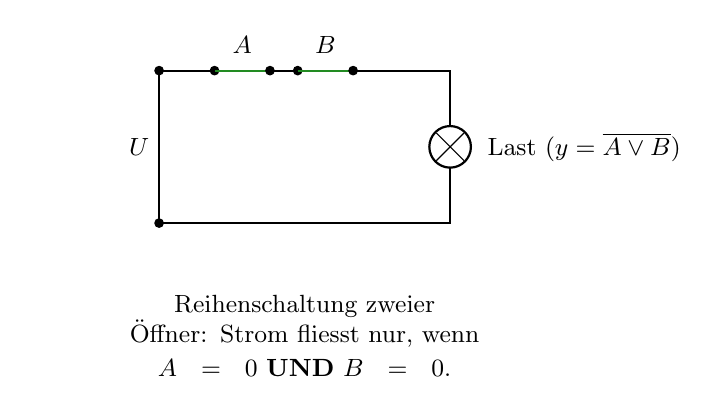
\begin{tikzpicture}[scale=0.88, >=stealth]
        \draw[thick] (0,0) -- (0,2.2) -- (0.8,2.2);
        \node[left, font=\small] at (0,1.1) {$U$};
        \fill (0,0) circle (2pt); \fill (0,2.2) circle (2pt);
        
        % Öffner A
        \fill (0.8, 2.2) circle (2pt);
        \draw[thick, ForestGreen] (0.8, 2.2) -- (1.6, 2.2);
        \node[above, font=\small] at (1.2, 2.3) {$A$};
        \fill (1.6, 2.2) circle (2pt);
        
        \draw[thick] (1.6, 2.2) -- (2.0, 2.2);
        
        % Öffner B
        \fill (2.0, 2.2) circle (2pt);
        \draw[thick, ForestGreen] (2.0, 2.2) -- (2.8, 2.2);
        \node[above, font=\small] at (2.4, 2.3) {$B$};
        \fill (2.8, 2.2) circle (2pt);
        
        \draw[thick] (2.8, 2.2) -- (4.2, 2.2) -- (4.2, 1.4);
        
        % Lampe y
        \draw[thick] (4.2, 1.1) circle (0.3);
        \draw (4.0, 0.9) -- (4.4, 1.3);
        \draw (4.0, 1.3) -- (4.4, 0.9);
        \node[right, font=\small] at (4.6, 1.1) {Last ($y = \overline{A \lor B}$)};
        \draw[thick] (4.2, 0.8) -- (4.2, 0) -- (0,0);
        
        \node[align=center, font=\small, text width=6.8cm, anchor=north] at (2.1, -0.9) {Reihenschaltung zweier Öffner: Strom fliesst nur, wenn\\[1pt]\textbf{$A=0$ UND $B=0$}.};
    \end{tikzpicture}
    \caption{Elektrische Schaltung für NOR: Reihenschaltung zweier Ruhekontakte (Öffner).}
    \label{fig:nor_schaltung}
\end{figure}

\begin{myexercise}
    Gegeben ist die Verknüpfung $\overline{x \vee y}$ (NOR). Bestimmen Sie das Ausgangssignal für folgende Eingangskombinationen:
    (1) $x=0, y=0$, (2) $x=1, y=0$, (3) $x=1, y=1$.
    \begin{myanswer}
        (1) $\overline{0 \vee 0} = 1$, (2) $\overline{1 \vee 0} = 0$, (3) $\overline{1 \vee 1} = 0$.
    \end{myanswer}
\end{myexercise}

\subsection{XOR -- Exklusiv-ODER (Antivalenz)}

\begin{mydefinition}[XOR-Gatter]
    Das \textbf{XOR-Gatter} (Exklusiv-ODER) liefert genau dann den Ausgang \texttt{1}, wenn sich die beiden Eingänge \emph{voneinander unterscheiden} ($x \neq y$):
    \[
        x \oplus y = 1 \iff (x = 1 \text{ und } y = 0) \text{ oder } (x = 0 \text{ und } y = 1).
    \]
\end{mydefinition}

\begin{figure}[H]
    \centering
    \begin{tikzpicture}[circuit logic US, scale=1.3]
    \node[xor gate, draw] (xor1) {};
    \draw (xor1.input 1) ++(-0.7,0) -- (xor1.input 1) node[left] {$x$};
    \draw (xor1.input 2) ++(-0.7,0) -- (xor1.input 2) node[left] {$y$};
    \draw (xor1.output) -- ++(0.7,0) node[right] {$x \oplus y$};
\end{tikzpicture}

    \caption{Symbol des XOR-Gatters.}
    \label{fig:xor_gatter}
\end{figure}

\begin{table}[H]
    \centering
    \begin{tabular}{ccc}
        $x$ & $y$ & $x \oplus y$ \\\midrule\midrule
        0 & 0 & 0 \\\midrule
        0 & 1 & 1 \\\midrule
        1 & 0 & 1 \\\midrule
        1 & 1 & 0 \\
    \end{tabular}
    \caption{Wahrheitstabelle des XOR-Gatters.}
    \label{tab:xor}
\end{table}

\begin{figure}[H]
    \centering
    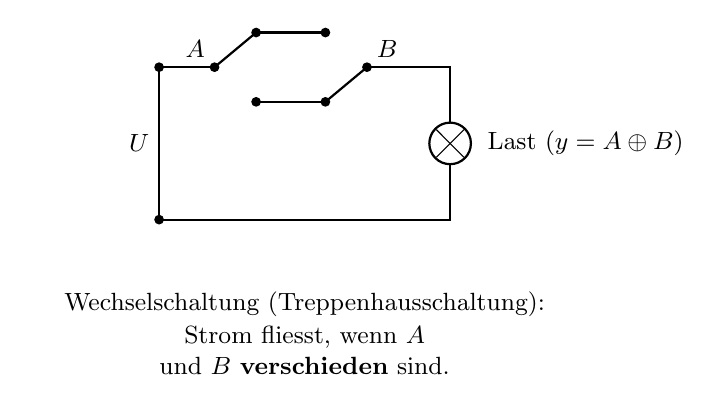
\begin{tikzpicture}[scale=0.88, >=stealth]
        \draw[thick] (0,0) -- (0,2.2) -- (0.8,2.2);
        \node[left, font=\small] at (0,1.1) {$U$};
        \fill (0,0) circle (2pt); \fill (0,2.2) circle (2pt);
        
        % Wechselschalter A
        \fill (0.8, 2.2) circle (2pt);
        \draw[thick] (0.8, 2.2) -- (1.4, 2.7);
        \node[above left, font=\small] at (0.8, 2.2) {$A$};
        \fill (1.4, 2.7) circle (2pt); \fill (1.4, 1.7) circle (2pt);
        \draw[thick] (1.4, 2.7) -- (2.4, 2.7);
        \draw[thick] (1.4, 1.7) -- (2.4, 1.7);
        
        % Wechselschalter B
        \fill (2.4, 2.7) circle (2pt); \fill (2.4, 1.7) circle (2pt);
        \draw[thick] (3.0, 2.2) -- (2.4, 1.7);
        \node[above right, font=\small] at (3.0, 2.2) {$B$};
        \fill (3.0, 2.2) circle (2pt);
        \draw[thick] (3.0, 2.2) -- (4.2, 2.2) -- (4.2, 1.4);
        
        % Lampe y
        \draw[thick] (4.2, 1.1) circle (0.3);
        \draw (4.0, 0.9) -- (4.4, 1.3);
        \draw (4.0, 1.3) -- (4.4, 0.9);
        \node[right, font=\small] at (4.6, 1.1) {Last ($y = A \oplus B$)};
        \draw[thick] (4.2, 0.8) -- (4.2, 0) -- (0,0);
        
        \node[align=center, font=\small, text width=6.8cm, anchor=north] at (2.1, -0.9) {Wechselschaltung (Treppenhausschaltung):\\[1pt]Strom fliesst, wenn $A$ und $B$ \textbf{verschieden} sind.};
    \end{tikzpicture}
    \caption{Elektrische Schaltung für XOR: Wechselschaltung mit zwei Umschaltern.}
    \label{fig:xor_schaltung}
\end{figure}

\begin{myexercise}
    In einem Flur soll das Licht über zwei Wechselschalter $A$ und $B$ (einer am Anfang, einer am Ende des Flurs) unabhängig voneinander ein- und ausgeschaltet werden können.
    Zeigen Sie anhand der Wechselschaltung in \cref{fig:xor_schaltung}, warum das Verhalten einer XOR-Verknüpfung entspricht.
    \begin{myanswer}
        Befinden sich beide Schalter in der gleichen Stellung ($0,0$ oder $1,1$), existiert kein geschlossener Strompfad. Wird einer der beiden Schalter umgelegt (Zustand ändert auf $0,1$ bzw. $1,0$), schliesst sich der Pfad und das Licht brennt. Umlegen eines beliebigen Schalters kehrt den Zustand der Lampe jeweils um.
    \end{myanswer}
\end{myexercise}

\section{Schaltkreise für die Binäraddition: Halbaddierer und Volladdierer}\label{sec:halbaddierer}

Wie verarbeitet eine digitale Schaltung (wie die \gls{ALU} in einer CPU) arithmetische Operationen? Das Herzstück jedes Prozessors ist die Fähigkeit, zwei Binärzahlen zu addieren. Bevor wir uns ansehen, wie dies mit Logikgattern gelöst wird, betrachten wir das Prinzip der binären Addition.

\subsection{Rechnen im Binärsystem}

Das Rechnen im Binärsystem funktioniert genauso, wie Sie es aus dem Dezimalsystem gewohnt sind: Stellenweise von rechts nach links addieren und bei Bedarf einen Übertrag (\textit{carry}) an die nächsthöhere Stelle weiterreichen.

Dabei gelten die folgenden Grundregeln für die Addition von zwei bzw. drei Bits:
\begin{itemize}
	\item $0 + 0 = 0$
	\item $0 + 1 = 1$
	\item $1 + 0 = 1$
	\item $1 + 1 = 0$, Übertrag $1$ \quad ($10_2 = 2_{10}$)
	\item $1 + 1 + 1 = 1$, Übertrag $1$ \quad ($11_2 = 3_{10}$)
\end{itemize}

Ein Beispiel für die schriftliche Addition zweier Binärzahlen:
\[
	\begin{array}{ccccccc}
		  & 1               & 0               & 1               & 0               & 1               & 1_2              \\
		+ & \underset{1}{1} & \underset{1}{1} & \underset{0}{1} & \underset{1}{0} & \underset{0}{1} & \underset{}{0_2} \\
		\hline
		1 & 1               & 0               & 0               & 1               & 0               & 1_2              \\\hline\hline
	\end{array}
\]

\begin{myexercise}
	Rechnen Sie die folgenden beiden Binärzahlen schriftlich zusammen: $10001010_2 + 11101_2$.
	\begin{myanswer}
		\[
			\begin{array}{ccccccccc}
				  & 1 & 0 & 0 & 0 & 1 & 0 & 1 & 0_2 \\
				+ & 0 & 0 & 0 & 1 & 1 & 1 & 0 & 1_2 \\
				\hline
				  & 1 & 0 & 1 & 0 & 0 & 1 & 1 & 1_2 \\
				\hline\hline
			\end{array}
		\]
		Dezimal-Kontrolle: $138_{10} + 29_{10} = 167_{10} = 10100111_2$.
	\end{myanswer}
\end{myexercise}

\begin{myexercise}\label{myexercise:overflow}
	Rechnen Sie folgende beiden Zahlen im Binärsystem zusammen: $11110001_2 + 00001111_2$.
	\begin{myanswer}
		Mathematisch korrekt ist $100000000_2$ ($256_{10}$). In einer festen 8-Bit-Umgebung (wie im Register/ALU eines 8-Bit-Prozessors) passt die 9. Stelle nicht mehr in das Register. Die vorderste $1$ geht verloren und das Resultat wird zu $00000000_2$. Man spricht von einem \tib{Überlauf}\index{Überlauf} (\textit{overflow}).
	\end{myanswer}
\end{myexercise}

\subsection{Der Halbaddierer}

Wie setzen wir dieses schriftliche Addieren nun in elektronischen Logikgattern um? Betrachten wir zunächst die Addition zweier einzelner Bits $x$ und $y$:
\begin{align*}
    0 + 0 &= 00_2 \quad (\text{Summe } 0, \text{ Übertrag } 0) \\
    0 + 1 &= 01_2 \quad (\text{Summe } 1, \text{ Übertrag } 0) \\
    1 + 0 &= 01_2 \quad (\text{Summe } 1, \text{ Übertrag } 0) \\
    1 + 1 &= 10_2 \quad (\text{Summe } 0, \text{ Übertrag } 1)
\end{align*}

Vergleicht man diese Ausgänge mit den bekannten Gattern, stellt man fest:
\begin{itemize}
    \item Die \textbf{Summe} $s$ entspricht exakt dem \textbf{XOR-Gatter}: $s = x \oplus y$.
    \item Der \textbf{Übertrag} $c$ (\textit{carry}) entspricht exakt dem \textbf{AND-Gatter}: $c = x \land y$.
\end{itemize}

Eine Schaltung, die zwei Bits $x$ und $y$ addiert und daraus ein Summenbit $s$ und ein Übertragsbit $c$ erzeugt, heisst \tib{Halbaddierer}\index{Halbaddierer}.

\begin{figure}[H]
    \centering
    \begin{tikzpicture}[circuit logic US, scale=1.2]
    \begin{scope}[local bounding box=haBB]
        \coordinate (ha-base) at (2,0.5);
        \coordinate (ha-and-pos) at ($(ha-base)+(0,-1.4)$);
        \node[xor gate, draw] (xor1) at (ha-base) {};
        \node[and gate, draw] (and1) at (ha-and-pos) {};

        \coordinate (ha-x-left) at ($(xor1.input 1)+(-1.2,0)$);
        \coordinate (ha-x-split) at ($(xor1.input 1)+(-0.5,0)$);
        \coordinate (ha-x-and) at ($(and1.input 1)+(-0.5,0)$);
        \draw (ha-x-left) -- (ha-x-split) -- (xor1.input 1);
        \draw (ha-x-split) -- ++(0,-0.5) -- (ha-x-and) -- (and1.input 1);
        \node[left] at (ha-x-left) {$x$};

        \coordinate (ha-y-left) at ($(xor1.input 2)+(-1.2,0)$);
        \coordinate (ha-y-split) at ($(xor1.input 2)+(-0.3,0)$);
        \coordinate (ha-y-and) at ($(and1.input 2)+(-0.3,0)$);
        \draw (ha-y-left) -- (ha-y-split) -- (xor1.input 2);
        \draw (ha-y-split) -- ++(0,-0.5) -- (ha-y-and) -- (and1.input 2);
        \node[left] at (ha-y-left) {$y$};

        \coordinate (ha-s-right) at ($(xor1.output)+(0.8,0)$);
        \coordinate (ha-c-right) at ($(and1.output)+(0.8,0)$);
        \draw (xor1.output) -- (ha-s-right) node[right] {$s$ (Summe)};
        \draw (and1.output) -- (ha-c-right) node[right] {$c$ (Übertrag)};
    \end{scope}
\end{tikzpicture}

    \caption{Schaltplan eines Halbaddierers: XOR liefert die Summe $s$, AND den Übertrag $c$.}
    \label{fig:halbaddierer}
\end{figure}

Zusammenfassend benötigt ein Halbaddierer genau \textbf{zwei Gatter}, um zwei 1-Bit-Zahlen $x$ und $y$ zu addieren:
\begin{itemize}
    \item \textbf{XOR-Gatter (Exklusiv-ODER)} für das Summenbit $s = x \oplus y$: Es liefert $1$, wenn genau ein Eingang $1$ ist.
    \item \textbf{AND-Gatter (UND)} für das Übertragsbit $c = x \land y$: Es liefert nur dann $1$, wenn beide Eingänge $1$ sind ($1+1 = 10_2 = 2_{10}$).
\end{itemize}

\begin{myexercise}
    Füllen Sie die Wahrheitstabelle des Halbaddierers für alle 4 Kombinationen von $x$ und $y$ aus. Berechnen Sie das Summenbit $s = x \oplus y$, das Übertragsbit $c = x \land y$, die zusammengesetzte 2-stellige Binärzahl $(c s)_2$ sowie deren Dezimalwert:
    \begin{center}
        \begin{tabular}{cccccc}
            $x$ & $y$ & Summe $s$ ($x \oplus y$) & Übertrag $c$ ($x \land y$) & Binärzahl $(c s)_2$ & Dezimalwert \\ \midrule\midrule
            0 & 0 & ? & ? & ? & ? \\ \midrule
            0 & 1 & ? & ? & ? & ? \\ \midrule
            1 & 0 & ? & ? & ? & ? \\ \midrule
            1 & 1 & ? & ? & ? & ? \\
        \end{tabular}
    \end{center}

    \begin{myanswer}
        \begin{center}
        \begin{tabular}{cccccc}
            $x$ & $y$ & Summe $s$ ($x \oplus y$) & Übertrag $c$ ($x \land y$) & Binärzahl $(c s)_2$ & Dezimalwert \\ \midrule\midrule
            0 & 0 & 0 & 0 & $00_2$ & $0_{10}$ \\ \midrule
            0 & 1 & 1 & 0 & $01_2$ & $1_{10}$ \\ \midrule
            1 & 0 & 1 & 0 & $01_2$ & $1_{10}$ \\ \midrule
            1 & 1 & 0 & 1 & $10_2$ & $2_{10}$ \\
        \end{tabular}
        \end{center}
    \end{myanswer}
\end{myexercise}

\subsection{Der Volladdierer}

Warum reicht ein Halbaddierer nicht aus, um zwei mehrstellige Binärzahlen (wie z.\,B. $1011_2 + 1101_2$) zu addieren? Beim schriftlichen Addieren mehrerer Stellen entsteht aus der vorherigen Stelle ein eingehender Übertrag $c_{\text{in}}$ (\textit{carry-in}), den die Schaltung ebenfalls mitverarbeiten muss!

Ein \tib{Volladdierer}\index{Volladdierer} besitzt daher \textbf{drei Eingänge} ($x$, $y$ sowie den eingehenden Übertrag $c_{\text{in}}$) und erzeugt wieder zwei Ausgänge: das Summenbit $s$ und den neuen Ausgangsübertrag $c_{\text{out}}$.

\begin{table}[H]
    \centering
    \begin{tabular}{ccccc}
        $x$ & $y$ & $c_{\text{in}}$ & Summe $s$ & Übertrag $c_{\text{out}}$ \\ \midrule\midrule
        0 & 0 & 0 & 0 & 0 \\ \midrule
        0 & 0 & 1 & 1 & 0 \\ \midrule
        0 & 1 & 0 & 1 & 0 \\ \midrule
        0 & 1 & 1 & 0 & 1 \\ \midrule
        1 & 0 & 0 & 1 & 0 \\ \midrule
        1 & 0 & 1 & 0 & 1 \\ \midrule
        1 & 1 & 0 & 0 & 1 \\ \midrule
        1 & 1 & 1 & 1 & 1 \\
    \end{tabular}
    \caption{Wahrheitstabelle des Volladdierers}
    \label{tab:volladdierer_wahrheitstabelle}
\end{table}

Ein Volladdierer lässt sich aus \textbf{zwei Halbaddierern} und einem \textbf{OR-Gatter} aufbauen:
Der erste Halbaddierer addiert $x$ und $y$. Der zweite Halbaddierer addiert das vorläufige Summenbit mit $c_{\text{in}}$. Ein OR-Gatter verknüpft die Überträge beider Halbaddierer zum finalen $c_{\text{out}}$.

\begin{figure}[H]
    \centering
    \begin{tikzpicture}[circuit logic US, scale=0.88, >=stealth]
    % Block 1: HA1
    \draw[thick, fill=gray!10, rounded corners=3pt] (0, 0) rectangle (1.8, 1.8);
    \node[font=\normalsize\bfseries] at (0.9, 0.9) {HA 1};
    
    % Block 2: HA2
    \draw[thick, fill=gray!10, rounded corners=3pt] (3.6, 0) rectangle (5.4, 1.8);
    \node[font=\normalsize\bfseries] at (4.5, 0.9) {HA 2};
    
    % OR Gate
    \node[or gate, draw, thick, fill=white] (or1) at (7.4, -0.9) {};

    % Inputs to HA 1
    \draw[thick, ->] (-0.8, 1.35) node[left] {$x$} -- (0, 1.35);
    \draw[thick, ->] (-0.8, 0.45) node[left] {$y$} -- (0, 0.45);
    
    % Sum line from HA 1 to HA 2
    \draw[thick, ->] (1.8, 1.35) -- node[above, font=\small] {$s_1$} (3.6, 1.35);
    
    % Carry-in line to HA 2
    \draw[thick, ->] (-0.8, -0.55) node[left] {$c_{\text{in}}$} -- (2.8, -0.55) |- (3.6, 0.45);
    
    % Final Sum line
    \draw[thick, ->] (5.4, 1.35) -- (9.2, 1.35) node[right] {\textbf{$s$ (Summe)}};
    
    % Carry 1 line (from HA 1 to OR gate input 2)
    \draw[thick] (1.8, 0.45) -- node[above, font=\small] {$c_1$} (2.2, 0.45) |- (or1.input 2);
    
    % Carry 2 line (from HA 2 to OR gate input 1)
    \draw[thick] (5.4, 0.45) -- node[above, font=\small] {$c_2$} (6.2, 0.45) |- (or1.input 1);
    
    % Final Carry-out line
    \draw[thick, ->] (or1.output) -- (9.2, -0.9) node[right] {\textbf{$c_{\text{out}}$ (Übertrag)}};
\end{tikzpicture}




    \caption{Aufbau eines Volladdierers aus zwei Halbaddierern (HA 1, HA 2) und einem OR-Gatter.}
    \label{fig:volladdierer_block}
\end{figure}

\subsection{Kaskadierung zum mehrstelligen Addierwerk (Ripple-Carry)}

Kaskadiert man $n$ Volladdierer hintereinander, indem man den Übertragsausgang $c_{\text{out}}$ jeder Stelle an den Übertragseingang $c_{\text{in}}$ der nächsthöheren Stelle weiterleitet, entsteht ein mehrstelliges Addierwerk (sogenannter \tib{Ripple-Carry-Addierer}\index{Ripple-Carry-Addierer}).

Genau diese Schaltung führt elektronisch die \textbf{schriftliche Addition im Binärsystem} aus: Jede Bitstelle (jede Spalte der schriftlichen Rechnung) wird von einem eigenen Volladdierer berechnet. Der Übertrag \enquote{plätschert} (\textit{ripples}) dabei von der niederwertigsten Stelle (Bit 0, ganz rechts) bis zur höchstwertigen Stelle (links) durch die Kette:

\begin{figure}[H]
    \centering
    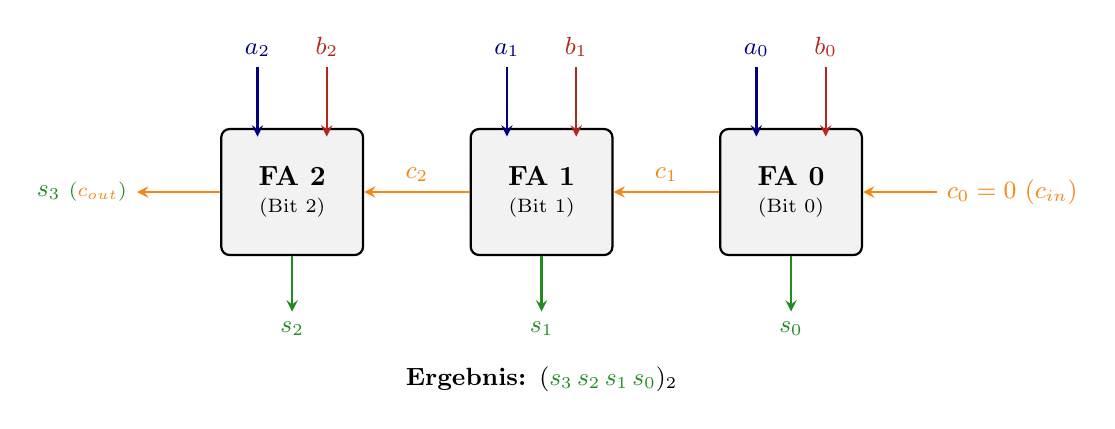
\begin{tikzpicture}[
    scale=0.88, >=stealth,
    fa/.style={draw, thick, fill=gray!10, rounded corners=3pt, minimum width=1.8cm, minimum height=1.6cm, align=center},
    wire/.style={thick, ->}
]
    % FA Blocks (Bit 2 on left, Bit 0 on right)
    \node[fa] (fa2) at (0, 0) {\textbf{FA 2}\\[-2pt]{\scriptsize (Bit 2)}};
    \node[fa] (fa1) at (3.6, 0) {\textbf{FA 1}\\[-2pt]{\scriptsize (Bit 1)}};
    \node[fa] (fa0) at (7.2, 0) {\textbf{FA 0}\\[-2pt]{\scriptsize (Bit 0)}};

    % Inputs from top (a_i in NavyBlue, b_i in BrickRed)
    \draw[wire, NavyBlue] (-0.5, 1.8) node[above, font=\small, NavyBlue] {$a_2$} -- (-0.5, 0.8);
    \draw[wire, BrickRed] (0.5, 1.8) node[above, font=\small, BrickRed] {$b_2$} -- (0.5, 0.8);

    \draw[wire, NavyBlue] (3.1, 1.8) node[above, font=\small, NavyBlue] {$a_1$} -- (3.1, 0.8);
    \draw[wire, BrickRed] (4.1, 1.8) node[above, font=\small, BrickRed] {$b_1$} -- (4.1, 0.8);

    \draw[wire, NavyBlue] (6.7, 1.8) node[above, font=\small, NavyBlue] {$a_0$} -- (6.7, 0.8);
    \draw[wire, BrickRed] (7.7, 1.8) node[above, font=\small, BrickRed] {$b_0$} -- (7.7, 0.8);

    % Carry chain in BurntOrange (from right to left)
    \draw[wire, BurntOrange] (9.3, 0) node[right, font=\small, BurntOrange] {$c_0 = 0$ ($c_{\text{in}}$)} -- (fa0.east);
    \draw[wire, BurntOrange] (fa0.west) -- node[above, font=\small, BurntOrange] {$c_1$} (fa1.east);
    \draw[wire, BurntOrange] (fa1.west) -- node[above, font=\small, BurntOrange] {$c_2$} (fa2.east);
    \draw[wire, BurntOrange] (fa2.west) -- ++(-1.2, 0) node[left, font=\small, ForestGreen] {\textbf{$s_3$} {\scriptsize (\textcolor{BurntOrange}{$c_{\text{out}}$})}};

    % Sum outputs in ForestGreen (to bottom)
    \draw[wire, ForestGreen] (fa2.south) -- ++(0, -0.8) node[below, font=\small, ForestGreen] {\textbf{$s_2$}};
    \draw[wire, ForestGreen] (fa1.south) -- ++(0, -0.8) node[below, font=\small, ForestGreen] {\textbf{$s_1$}};
    \draw[wire, ForestGreen] (fa0.south) -- ++(0, -0.8) node[below, font=\small, ForestGreen] {\textbf{$s_0$}};

    % Summary label
    \node[font=\small\bfseries, align=center] at (3.6, -2.7) {Ergebnis: $(\textcolor{ForestGreen}{s_3 \, s_2 \, s_1 \, s_0})_2$};
\end{tikzpicture}

    \caption{Kaskadierung von 3 Volladdierern (FA 0, FA 1, FA 2) zu einem 3-Bit-Ripple-Carry-Addierer.}
    \label{fig:ripple_carry_addierer}
\end{figure}

\begin{myremark}[Warum heisst es \enquote{Ripple-Carry}?]
    Der Name setzt sich aus zwei englischen Begriffen zusammen:
    \begin{itemize}
        \item \textbf{Carry (Übertrag):} Bezeichnet den beim Addieren entstehenden Übertrag, der an die nächsthöhere Bitstelle weitergereicht werden muss.
        \item \textbf{Ripple (Kräuseln / Wellenbewegung):} Da der Ausgangsübertrag $\textcolor{BurntOrange}{c_{\text{out}}}$ jeder Stufe den Eingang $\textcolor{BurntOrange}{c_{\text{in}}}$ der nächsten Stufe speist, kann ein Volladdierer sein stabiles Ergebnis erst dann berechnen, wenn das Übertragssignal der vorherigen Stufe bereitsteht. Im ungünstigsten Fall (z.\,B. bei $\textcolor{NavyBlue}{111_2} + \textcolor{BrickRed}{001_2} = \textcolor{ForestGreen}{1000_2}$) muss der Übertrag nacheinander wie eine Welle durch die gesamte Kette \enquote{durchplätschern} (\textit{ripple through}).
    \end{itemize}
    Die Signallaufzeit wächst daher linear mit der Anzahl der Bits ($O(n)$). In modernen Hochleistungsprozessoren kommen für breitere Zahlen (z.\,B. 32 oder 64 Bit) vorausschauende Addierwerke zum Einsatz (wie der \textit{Carry-Lookahead-Addierer}), welche alle Überträge parallel ermitteln.
\end{myremark}

\begin{myexercise}
    Gegeben ist die Addition der beiden 3-Bit-Zahlen $\textcolor{NavyBlue}{A = 011_2}$ ($3_{10}$) und $\textcolor{BrickRed}{B = 010_2}$ ($2_{10}$) mit dem eingehenden Übertrag $\textcolor{BurntOrange}{c_0 = 0}$.
    Bestimmen Sie für jeden der drei Volladdierer (FA 0, FA 1, FA 2) die Summenbits $\textcolor{ForestGreen}{s_0, s_1, s_2}$ sowie die weitergereichten Überträge $\textcolor{BurntOrange}{c_1, c_2, s_3}$:

    \begin{center}
        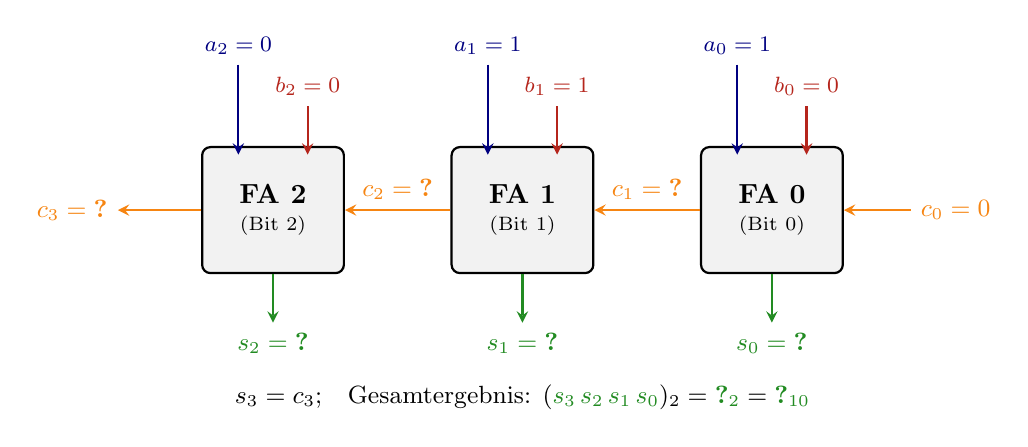
\begin{tikzpicture}[
    scale=0.88, >=stealth,
    fa/.style={draw, thick, fill=gray!10, rounded corners=3pt, minimum width=1.8cm, minimum height=1.6cm, align=center}
]
    % FA Blocks
    \node[fa] (fa2) at (0, 0) {\textbf{FA 2}\\[-2pt]{\scriptsize (Bit 2)}};
    \node[fa] (fa1) at (3.6, 0) {\textbf{FA 1}\\[-2pt]{\scriptsize (Bit 1)}};
    \node[fa] (fa0) at (7.2, 0) {\textbf{FA 0}\\[-2pt]{\scriptsize (Bit 0)}};

    % Inputs from top (a_i in NavyBlue, b_i in BrickRed)
    \draw[thick, ->, NavyBlue] (-0.5, 2.1) node[above, font=\footnotesize, NavyBlue] {$a_2 = 0$} -- (-0.5, 0.8);
    \draw[thick, ->, BrickRed] (0.5, 1.5) node[above, font=\footnotesize, BrickRed] {$b_2 = 0$} -- (0.5, 0.8);

    \draw[thick, ->, NavyBlue] (3.1, 2.1) node[above, font=\footnotesize, NavyBlue] {$a_1 = 1$} -- (3.1, 0.8);
    \draw[thick, ->, BrickRed] (4.1, 1.5) node[above, font=\footnotesize, BrickRed] {$b_1 = 1$} -- (4.1, 0.8);

    \draw[thick, ->, NavyBlue] (6.7, 2.1) node[above, font=\footnotesize, NavyBlue] {$a_0 = 1$} -- (6.7, 0.8);
    \draw[thick, ->, BrickRed] (7.7, 1.5) node[above, font=\footnotesize, BrickRed] {$b_0 = 0$} -- (7.7, 0.8);

    % Carry chain in BurntOrange (right to left)
    \draw[thick, ->, BurntOrange] (9.2, 0) node[right, font=\small, BurntOrange] {$c_0 = 0$} -- (fa0.east);
    \draw[thick, ->, BurntOrange] (fa0.west) -- (fa1.east) node[midway, above, font=\small, BurntOrange] {$c_1 = \textbf{?}$};
    \draw[thick, ->, BurntOrange] (fa1.west) -- (fa2.east) node[midway, above, font=\small, BurntOrange] {$c_2 = \textbf{?}$};
    \draw[thick, ->, BurntOrange] (fa2.west) -- ++(-1.2, 0) node[left, font=\small, BurntOrange] {$c_3 = \textbf{?}$};

    % Sum outputs in ForestGreen (to bottom)
    \draw[thick, ->, ForestGreen] (fa2.south) -- ++(0, -0.7) node[below, font=\small, ForestGreen] {$s_2 = \textbf{?}$};
    \draw[thick, ->, ForestGreen] (fa1.south) -- ++(0, -0.7) node[below, font=\small, ForestGreen] {$s_1 = \textbf{?}$};
    \draw[thick, ->, ForestGreen] (fa0.south) -- ++(0, -0.7) node[below, font=\small, ForestGreen] {$s_0 = \textbf{?}$};

    % Result line (spaced well below sum outputs)
    \node[font=\small, align=center] at (3.6, -2.7) {$s_3=c_3$;\quad Gesamtergebnis: $(\textcolor{ForestGreen}{s_3 \, s_2 \, s_1 \, s_0})_2 = \textcolor{ForestGreen}{\textbf{?}_2} = \textcolor{ForestGreen}{\textbf{?}_{10}}$};
\end{tikzpicture}

    \end{center}

    Führen Sie anschliessend die schriftliche Rechnung auch für die Aufgaben 2 und 3 durch und kontrollieren Sie im Dezimalsystem:
    \begin{center}
        \begin{tabular}{cccc}
            & \textbf{Aufgabe 1} & \textbf{Aufgabe 2} & \textbf{Aufgabe 3} \\ \midrule\midrule
            Zahl $\textcolor{NavyBlue}{A}$ (dezimal) & $3_{10}$ & $5_{10}$ & $7_{10}$ \\
            Zahl $\textcolor{BrickRed}{B}$ (dezimal) & $2_{10}$ & $3_{10}$ & $1_{10}$ \\ \midrule
            $\textcolor{NavyBlue}{A = a_2 a_1 a_0}$ & $\textcolor{NavyBlue}{011_2}$ & $\textcolor{NavyBlue}{101_2}$ & $\textcolor{NavyBlue}{111_2}$ \\
            $\textcolor{BrickRed}{B = b_2 b_1 b_0}$ & $\textcolor{BrickRed}{010_2}$ & $\textcolor{BrickRed}{011_2}$ & $\textcolor{BrickRed}{001_2}$ \\ \midrule
            $\textcolor{BurntOrange}{\text{Überträge } c_2 c_1 c_0}$ & ? & ? & ? \\
            $\textcolor{ForestGreen}{\text{Ergebnis } s_3 s_2 s_1 s_0}$ & ? & ? & ? \\ \midrule
            Dezimal-Kontrolle & ? & ? & ? \\
        \end{tabular}
    \end{center}

    \begin{myanswer}
        \textbf{Schrittweise Berechnung für Aufgabe 1 ($\textcolor{NavyBlue}{011_2} + \textcolor{BrickRed}{010_2}$, $\textcolor{BurntOrange}{c_0 = 0}$):}
        \begin{itemize}
            \item \textbf{FA 0 (Bit 0):} $\textcolor{NavyBlue}{a_0 = 1}, \textcolor{BrickRed}{b_0 = 0}, \textcolor{BurntOrange}{c_0 = 0} \implies \textcolor{ForestGreen}{s_0 = \mathbf{1}}, \textcolor{BurntOrange}{c_1 = \mathbf{0}}$
            \item \textbf{FA 1 (Bit 1):} $\textcolor{NavyBlue}{a_1 = 1}, \textcolor{BrickRed}{b_1 = 1}, \textcolor{BurntOrange}{c_1 = 0} \implies \textcolor{ForestGreen}{s_1 = \mathbf{0}}, \textcolor{BurntOrange}{c_2 = \mathbf{1}}$
            \item \textbf{FA 2 (Bit 2):} $\textcolor{NavyBlue}{a_2 = 0}, \textcolor{BrickRed}{b_2 = 0}, \textcolor{BurntOrange}{c_2 = 1} \implies \textcolor{ForestGreen}{s_2 = \mathbf{1}}, \textcolor{ForestGreen}{s_3} (\textcolor{BurntOrange}{c_{\text{out}}}) = \mathbf{0}$
            \item \textbf{Gesamtergebnis:} $(\textcolor{ForestGreen}{s_3 s_2 s_1 s_0})_2 = \textcolor{ForestGreen}{\mathbf{0101_2}} = \mathbf{5_{10}}$
        \end{itemize}
        \vspace{2mm}
        \textbf{Übersicht aller drei Aufgaben:}
        \begin{center}
        \begin{tabular}{cccc}
            & \textbf{Aufgabe 1} & \textbf{Aufgabe 2} & \textbf{Aufgabe 3} \\ \midrule\midrule
            $\textcolor{NavyBlue}{A}$ & $\textcolor{NavyBlue}{011_2 \ (3)}$ & $\textcolor{NavyBlue}{101_2 \ (5)}$ & $\textcolor{NavyBlue}{111_2 \ (7)}$ \\
            $\textcolor{BrickRed}{B}$ & $\textcolor{BrickRed}{010_2 \ (2)}$ & $\textcolor{BrickRed}{011_2 \ (3)}$ & $\textcolor{BrickRed}{001_2 \ (1)}$ \\ \midrule
            $\textcolor{BurntOrange}{\text{Überträge } c}$ & $\textcolor{BurntOrange}{010_2}$ & $\textcolor{BurntOrange}{111_2}$ & $\textcolor{BurntOrange}{111_2}$ \\
            $\textcolor{ForestGreen}{\text{Ergebnis } S}$ & $\textcolor{ForestGreen}{0101_2 \ (5_{10})}$ & $\textcolor{ForestGreen}{1000_2 \ (8_{10})}$ & $\textcolor{ForestGreen}{1000_2 \ (8_{10})}$ \\ \midrule
            Kontrolle & $3 + 2 = 5$ \checkmark & $5 + 3 = 8$ \checkmark & $7 + 1 = 8$ \checkmark \\
        \end{tabular}
        \end{center}
    \end{myanswer}
\end{myexercise}

Wir haben nun gesehen, wie aus einzelnen Transistoren Gatter, und aus Gattern vollwertige Rechenschaltungen wie der Halb- und Volladdierer entstehen. Im nächsten Kapitel betrachten wir, wie aus solchen Bausteinen ein vollständiger Computer aufgebaut wird.
